\section{Модификация проекта «Изображение проекции полиэдра»}

\subsection*{Точная постановка задачи}
Модифицируйте эталонный проект таким образом, 
чтобы определялась и печаталась следующая характеристика полиэдра: 
сумма длин проекций невидимых частей частично видимых рёбер, образующих с горизонтальной плоскостью угол не более $\pi/7$, центр которых находится 
строго внутри сферы $x^2+y^2+z^2=4$.


\subsection*{Решение данной задачи}
Чтобы успешно решить данную задачу необходимо изменить код в файлах $\texttt{shadow/polyedr.rb}$, $\texttt{common/polyedr.rb}$ и $\texttt{shadow/run\_polyedr.rb}$
Методы проверки ребра на частичную видимость, на проверку угла наклона к горизонтальной плоскости, на попадание центра ребра в заданную 
сферу и для вычисления длины проекции выполняется в методе $\texttt{magic}$ класса $\texttt{Polyedr}$ в файле $\texttt{shadow/polyedr.rb}$:


\begin{small}
\begin{verbatim}
class Polyedr 
  ...
 def magic()
    result = 0
    my_edges=edges.dup
    my_edges.each{|e| facets.each{|f| e.shadow(f)}}.uniq!
    my_edges.each do |e|
      if e.is_good?
        last=0.0
        e.gaps.each{|s| result+=e.r3(last).proection(e.r3(s.beg)); last=s.fin}
        result+=e.r3(last).proection(e.r3(1.0))
      end
    end
    result
  end
\end{verbatim}
\end{small}

 \subsection*{Модификация кода}

В файле $\texttt{common/polyedr.rb}$ дополним инициализацию и добавим методы в классе 
$\texttt{Edge}$. Объекты этого класса теперь будут хранить коэффициент гомотетии. Чтобы модификация не портила прохождение тестов для эталонного проекта, мы сделаем аргумент $\texttt{coef}$ по умолчанию равным единице:


\begin{small}
\begin{verbatim}
class Edge 
  ...
  def initialize(b, f, coef=1.0)
    @beg, @fin, @coef = b, f, coef
  end  
    ...
end
\end{verbatim}
\end{small}

Так как в некоторых фигурах (например, в кубе) одно и то же ребро может принадлежать разным граням, необходимо реализовать метод $\texttt{uniq}$ для класса $\texttt{Edge}$. Для этого нужно добавить 2 метода $\texttt{eql?}$ и $\texttt{hash}$:

\begin{small}
\begin{verbatim}
class Edge 
  ...
  def eql?(other)
    (@beg==other.beg && @fin==other.fin) or (@beg==other.fin && @fin==other.beg) 
  end
  def hash
    @beg.hash + @fin.hash
  end
end
\end{verbatim}
\end{small}

В данной реализации приметяется оператор $\texttt{==}$ для объектов класса $\texttt{R3}$, где этот метод не реализован. Чтобы этот оператор работал в классе $\texttt{R3}$ добавим метод  $\texttt{eql?}$:

\begin{small}
\begin{verbatim}
class R3
  ...
  def eql?(other)
    @x==other.x && @y==other.y && @z==other.z
  end
end
\end{verbatim}
\end{small}

Для выяснения, больше ли угол наклона к горизонтальной плоскости чем $\pi/7$, реализуем метод $\texttt{angle\_with\_xy}$. В данном методе используется метод $\texttt{atan}$ библиотеки математических функций Ruby $\texttt{Math}$. Этот метод возвращает арктангенс угла. В нашем случае, арктангенс нужного нам угла находится как отношение координаты z к проекции на плоскость Oxy. Метод $\texttt{atan}$ возвращает значения в диапазоне $\left [ -\pi/2,~\pi/2 \right ]$.

\begin{small}
\begin{verbatim}
class R3
  ...
  def angle_with_xy
    atan(@z/sqrt(@x**2+@y**2))<=::PI/7
  end
  ...
end
\end{verbatim}
\end{small}

Так же добавим метод $\texttt{proection(other)}$, который будет вычислять длину проекции отрезка, в котором началом является объект класса $\texttt{R3}$, от которого вызывается метод, а концом "--- объект класса $\texttt{R3}$, который передается в качестве аргумента.

\newpage
\begin{small}
\begin{verbatim}
class R3
  ...
  def proection(other)
    sqrt((other.x-@x)**2+(other.y-@y)**2)
  end
  ...
end
\end{verbatim}
\end{small}

На этом модификация файла $\texttt{common/polyedr.rb}$ завершена.Теперь необходимо модифицировать файл $\texttt{swadow/polyedr.rb}$.

  Для проверки ребра на частичную видимость необходимо проверить массив $\texttt{@gaps}$. Так как элементами массива $\texttt{@gaps}$ являются объекты класса $\texttt{Segment}$ и в этом классе есть доступ к чтению аттрибутов $\texttt{beg}$ и $\texttt{fin}$, которые соответственно являются началом и концом видимого отрезка, то мы можем получить эти значения. Значения  $\texttt{beg}$ и $\texttt{fin}$ могут варьироваться в промежутке от [0,1]. В методе $\texttt{is\_good?}$ мы суммируем длины всех видимых участков и если сумма не равна нулю (полностью невидимое ребро) и не равна 1(полностью видимое ребро), то проверяемое ребро является частично видимым. Так как вычисления производятся на компьютере, используется погрешность 0.000001:

\begin{small}
\begin{verbatim}
class Edge 
  ...
  def is_good?()
    sum=0
    @gaps.each{|x| sum=+x.fin-x.beg}
    sum > 0.000001 && sum < 0.999999
  end
  ...
end
\end{verbatim}
\end{small}

  Проверку центра ребра на принадлежность сфере реализует метод  $\texttt{is\_center\_good?}$ из класса $\texttt{Edge}$. Он базируется на базовых знаниях векторной алгебры. Координаты середины отрезка $[ \mathit a, \mathit b ]$ вычисляются по формуле: 
$$\frac{a_{x}+b_{x}}{2};~\frac{a_{y}+b_{y}}{2};~ \frac{a_{z}+b_{z}}{2}.$$

Из-за коэффициента гомотетии вероятность того, что центр ребра попадет в сферу радиуса 4, становится очень малой, поэтому мы делим каждую координату на коэффициент гомотетии.
\begin{small}
\begin{verbatim} 
  def is_center_good?()
    xc = (@beg.x + @fin.x) / (2.0*@coef)
    yc = (@beg.y + @fin.y) / (2.0*@coef)
    zc = (@beg.z + @fin.z) / (2.0*@coef)
    return ((xc**2+yc**2+zc**2)<4)
  end
\end{verbatim}
\end{small}

На этом модификация файла $\texttt{shadow/polyedr.rb}$ завершена.
Последняя модификация в файле $\texttt{shadow/run\_polyedr.rb}$ $-$ вывод результата на экран:

\begin{small}
\begin{verbatim}
#!/usr/bin/env ruby
require_relative './polyedr'
require_relative '../common/tk_drawer'
TkDrawer.create
%w(ccc box cube king).each do |name|
  puts '============================================================='
  puts "Начало работы с полиэдром '#{name}'"
  start_time = Time.now
  a=Polyedr.new("../data/#{name}.geom")
  a.draw
  puts "summ = #{a.magic}"
  puts "Изображение полиэдра '#{name}' заняло #{Time.now - start_time} сек."
  print 'Hit "Return" to continue -> '
  gets
end
\end{verbatim}
\end{small}

Модификация эталонного проекта «Изображение проекции полиэдра» завершена. Пример работы программы 
с модифицированным файлом $\texttt{test1.geom}$ можно увидеть на рис.2 и его содержание представленно ниже.
\begin{figure}[ht!]
\begin{center}
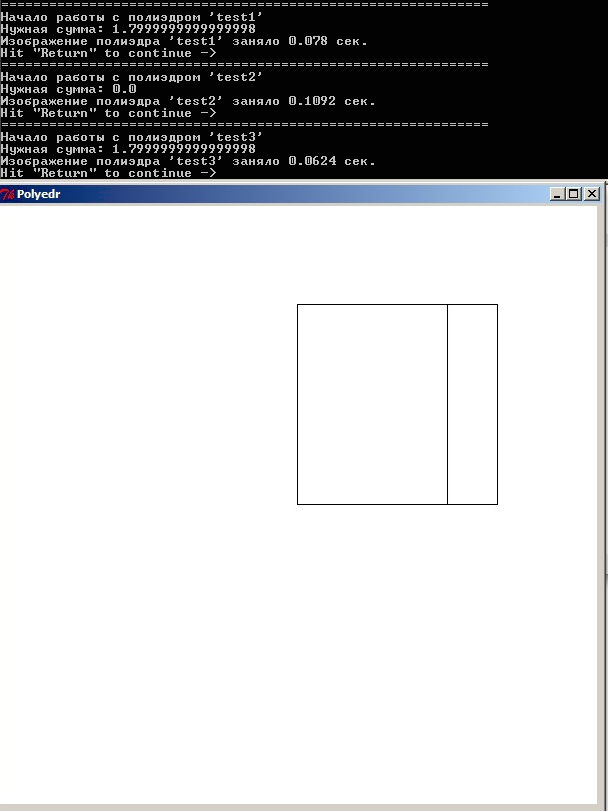
\includegraphics[width=0.8\hsize]{images/shadow}
\end{center}
\caption{Работа программы «Изображение проекции полиэдра»}
\end{figure}
\newpage\begin{small}
\begin{verbatim}
200.0	0 0 0
12	12	36
-1	-1	0	
-1	1	0	
1	1	0	
1	-1	0	
-0.5	-1	0.23
-0.5	1	0.23	
0.5	1	0.23	
0.5	-1	0.23
-0.75	-1	0.23
-0.75	1	0.23	
0.75	1	0.23	
0.75	-1	0.23
3 1 2 3
3 1 4 3
3 1 2 6  
3 1 5 6
3 1 4 8
3 1 5 8
3 4 3 7
3 4 8 7
3 2 3 7
3 2 6 7
3 9 10 11
3 9 12 11

\end{verbatim}
\end{small}



